การเคลื่อนที่แบบวงกลม  เป็นการเคลื่อนที่ในแนวโค้งรอบจุดศูนย์กลางจุดหนึ่ง   เช่นการเคลื่อนที่ของวัตถุที่ผูกไว้ด้วยเชือกแล้วเหวี่ยงให้เคลื่อนที่เป็นวงกลม   ,   การเคลื่อนที่ของรถไฟเหาะตีลังกา  ,   การเลี้ยวโค้งบนถนนของรถ   หรือการโคจรของดวงจันทร์รอบโลก  เป็นต้น
\begin{center}
\begin{minipage}{.45\textwidth}
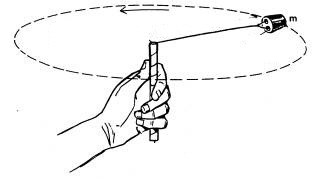
\includegraphics[width=\textwidth]{content-10-1.jpg}
\end{minipage} \hfill
\begin{minipage}{.45\textwidth}
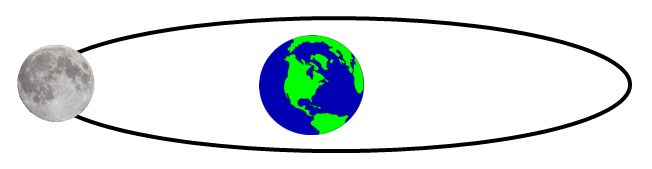
\includegraphics[width=\textwidth]{content-10-2.jpg}
\end{minipage}
\end{center}
\begin{center}
\begin{minipage}{.45\textwidth}
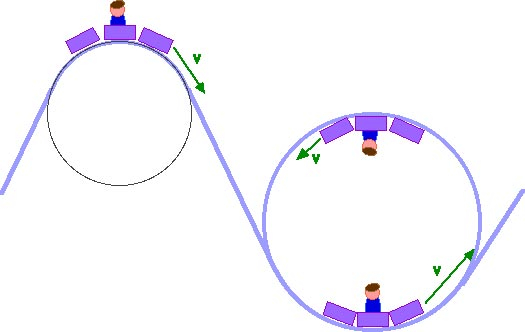
\includegraphics[width=\textwidth]{content-10-3.jpg}
\end{minipage} \hfill
\begin{minipage}{.45\textwidth}
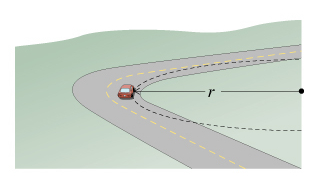
\includegraphics[width=\textwidth]{content-10-4.jpg}
\end{minipage}
\end{center}
